% Slide 10: Implementation Strategy
\begin{frame}{How We Implement}
    \framesubtitle{Our Proven Methodology}

    \begin{center}
        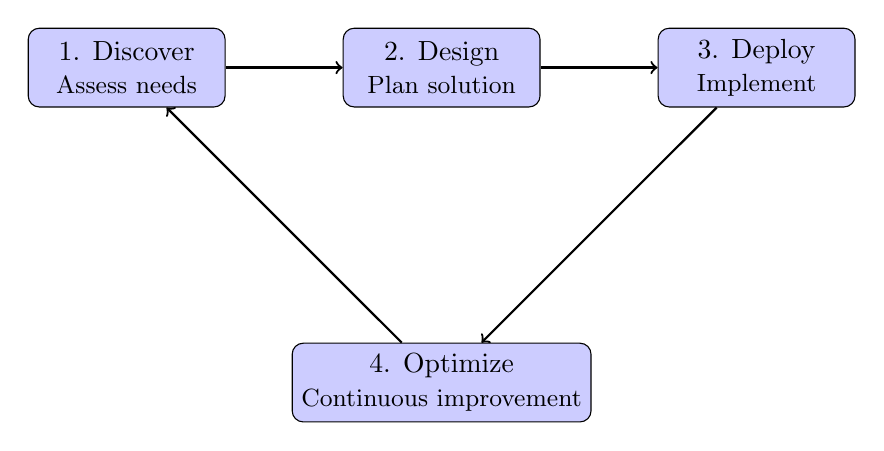
\begin{tikzpicture}[
            node distance=4cm,
            box/.style={rectangle,draw,fill=blue!20,rounded corners,minimum width=2.5cm,minimum height=1cm,align=center}
        ]
            \node[box] (discover) {1. Discover\\{\small Assess needs}};
            \node[box,right of=discover] (design) {2. Design\\{\small Plan solution}};
            \node[box,right of=design] (deploy) {3. Deploy\\{\small Implement}};
            \node[box,below of=design] (optimize) {4. Optimize\\{\small Continuous improvement}};

            \draw[->,thick] (discover) -- (design);
            \draw[->,thick] (design) -- (deploy);
            \draw[->,thick] (deploy) -- (optimize);
            \draw[->,thick] (optimize) -- (discover);
        \end{tikzpicture}
    \end{center}

    \vspace{0.3cm}

    \begin{columns}[t]
        \begin{column}{0.3\textwidth}
            \textbf{Technical Implementation:}
            \begin{itemize}
                \item Cloud-native architecture
                \item Microservices design
                \item API-first approach
                \item Automated CI/CD pipeline
            \end{itemize}
        \end{column}

        \begin{column}{0.3\textwidth}
            \textbf{Customer Success:}
            \begin{itemize}
                \item Dedicated onboarding team
                \item 90-day success program
                \item Regular training sessions
                \item Quarterly business reviews
            \end{itemize}
        \end{column}
    \end{columns}
\end{frame}
